\section{Регрессионное тестирование}

Для того чтобы знать, какие тесты перезапускать после того или иного изменения в программе, нужно определить, от каких конкретно частей программы (модулей, методов, и т.п.) зависит результат каждого теста. Для этого часто используется ​управляющий граф​, отображающий поток управления программы, по которому легко отследить зависимости одних блоков/модулей/методов от других.

Web-приложения строятся по принципу микросервисной архитектуры. Поэтому составные модули веб-приложений должны быть независимыми. Более того, методы-обработчики http запросов в этих модулях - также часто не зависят друг от друга. Поэтому на каждый метод-обработчик пишется несколько тестов, которые проверяют качество данного метода. А учитывая специфику веб-приложений, эти тесты никак не будут связанны с другими методами. Из этого я могу сделать вывод, что строить матрицу тестов-методов н имеет смысла (т.к. каждый тест проверяет определенный метод и ни как не связан с другими методами).

Мои одногруппники успешно сдавали регрессионное тестирование как раз на уровне методов. Т.е. строили матрицу зависимости метода от теста. Однако я уже показал, что в моём приложении данный подход не имеет смысла. 

На лекции регрессионное тестирование объяснялось на уровне кода. Т.е. я это понимаю так: мы можем взять один метод, взять тесты, которые написаны для этого теста, построить граф потока управления данного метода, построить зависимости узлов графа(строчек кода) от тестов этого метода и из этого сделать вывод, какие тесты необходимо запускать, при изменении определенной строчки кода, а какие нет.

Рассмотрим данный подход на примере метода \textbf{/set-info} модуля \textbf{referee.js}

\textbf{/set-info} получает событие, произошедшее в заданном матче с описанием события.

Для данного метода из раздела \ref{subsec:referee-test} описаны тесты:
\begin{enumerate}
	\item отправка события \textbf{MATCH\_STARTED} в существующем матче
	\item отправка события \textbf{MATCH\_FINISHED} в существующем матче
	\item отправка любого события по несуществующиму id
	\item отправка любого события c отсутствующим полем id в запросе
\end{enumerate}

\begin{lstlisting}[caption={Код метода обработчика урла /set-info}, label={lst:set-info}]
router.post('/set-info', function(req, res, next) {
    let idMatch = req.body.idMatch;
    let idEvent = req.body.idEvent;
    let idAction = req.body.idAction;
    let minute = req.body.minute;

    if (!idMatch || !idEvent || isNaN(idAction) || isNaN(minute)) {
        return res.status(400).json(null);
    }

    let now = new Date();

    let event = {
        idEvent: idEvent,
        idAction: idAction,
        minute: minute,
        realTime: now,
    };

    Match.findById(idMatch, function (err, match) {
        if (err || !match) {
            return res.status(404).json(null);
        }

        switch (idEvent) {
            case Match.EVENT.MATCH_STARTED.name:
                match.status = Match.STATUS.RUNNING.name;
                break;
            case Match.EVENT.MATCH_FINISHED.name:
                match.status = Match.STATUS.FINISHED.name;
                break;
            case Match.EVENT.GOAL.name:
            case Match.EVENT.OWN_GOAL.name:
            case Match.EVENT.YELLOW_CARD.name:
            case Match.EVENT.RED_CARD.name:
                event.idTeam = req.body.idTeam;
                event.idPlayer = req.body.idPlayer;
                event.teamName = req.body.teamName;
                event.playerName = req.body.playerName;
                break;

        }

        match.events.push(event);

        clients.forEach((ws) => {
            ws.send(JSON.stringify(event));
        });

        match.save(function (err) {
            if (err) {
                return res.status(500).json(null);
            }

            return res.status(200).json(null);
        });
    });
});
\end{lstlisting}

По листингу \ref{lst:set-info} построим граф потока управления. Каждый узел графа (блок) отмечен заглавной латинской буквой. Числа в скобках указывают на строчки кода в листинге \ref{lst:set-info}.

\begin{figure}[H]
  \centering
  \includegraphics[scale=0.8]{graph-set-info.png}
  \caption{Граф потока управления метода обработчика /set-info}
\end{figure}

\begin{table}[H] 
\caption{\label{tab:block_graph-test} Матрица зависимостей блоков графа от тестов}
\begin{center}
\begin{tabular}{|l|c|c|c|c|}

\hline
 & \multicolumn{4}{|c|}{тесты} \\
\hline
блок & a & б & в & г\\
\hline
A & - & - & - & -\\
\hline
B & - & - & - & +\\
\hline
C & - & - & - & -\\
\hline
D & - & - & + & -\\
\hline
E & - & - & - & -\\
\hline
F & + & - & - & -\\
\hline
G & - & + & - & -\\
\hline
H & - & - & - & -\\
\hline
I & - & - & - & -\\
\hline
J & - & - & - & -\\
\hline
K & + & + & - & -\\
\hline
\end{tabular}
\end{center}
\end{table} 

Для проверки правильности составленной таблицы \ref{tab:block_graph-test} изменим строчку №55, которая соответствует блоку K. 

\begin{figure}[H]
  \centering
  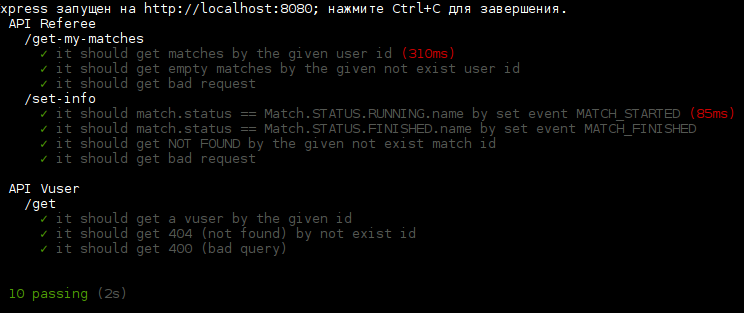
\includegraphics[scale=1]{screen1.png}
  \caption{Прохождение тестов до изменения блока K}
  \label{image:before-edit}
\end{figure}

\begin{figure}[H]
  \centering
  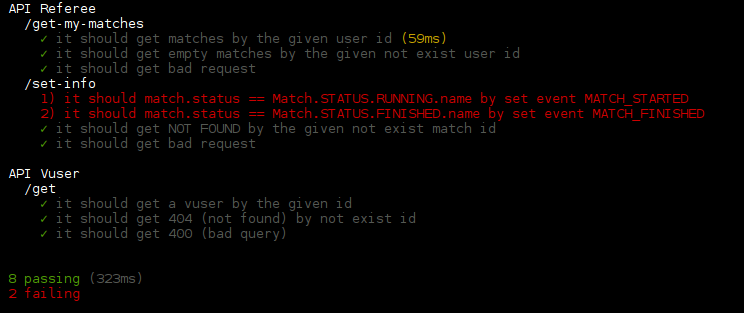
\includegraphics[scale=1]{screen2.png}
  \caption{Прохождение тестов после изменения блока K}
  \label{image:after-edit}
\end{figure}

По рисункам \ref{image:before-edit} и \ref{image:after-edit} видно, что после изменения блока K стали падать тесты a, б, что соответствует построенной таблице \ref{tab:block_graph-test}
